%\documentclass[10pt]{article}
%\usepackage{graphicx}
%\usepackage{amsmath}
%\usepackage{fullpage}
%\usepackage[icelandic]{babel}
%\usepackage[T1]{fontenc}
%\usepackage[utf8x]{inputenc}	
%
%\title{Forecasting Models}
%\author{David Erik Mollberg \and Guðjón Ingibergur Ólafsson \and Gunnar Gylfason \and Magnea Gunnarsdóttir \and Rebekka Jóhannsdóttir \and Róbert Árnason \and Steindór Tryggvason \and Styrmir Gauti Fjeldsted \and Vésteinn Sigurjónsson}
%
%\begin{document}
%\maketitle

\section {Sveiflur og letni(e.trends)}
 
Þegar spá þarf fyrir um sveiflur eða leitni sem eru í gangi þá þarf að passa að velja réttar spáaðferðir. Gagnlegt er að líta á vöxt fyrirtækinsins og markaðarins í sölu/aðgerðum, þegar litið er á gögn um mánaða eða árabil og augljóst mynstur er milli daga, vikna eða mánaða má áætla að mynstrið haldi áfram og hægt að yfirfara það í spá. Mikilvægt að hafa næg gögn yfirleitt miðað við tvö tímabil eða meira. \cite{What-Is-Trend-Forecasting}

%\subsection{Figures}
%
%\begin{figure}[htb]
%\begin{center}
%
%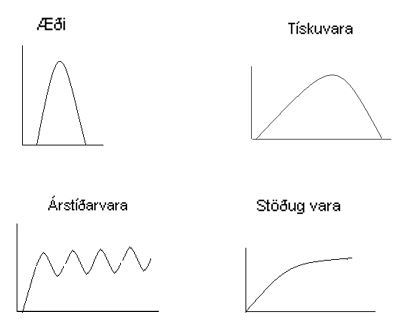
\includegraphics[width=0.75\textwidth]{tegundirspar}
%\caption{Mismunandi eftirspurn sem þarf að spá fyrir}
%\label{fig:figure1}
%\end{center}
%\end{figure}

\subsection{Aðferðir}
Árstíðarsveiflur eða vikusveiflu geta verið metna með árstíðarsveiflustðulum (e.seasonal index), getur verið háð eða óháð breytingu á meðal eftirspurnar. Leitni (e.trend) er auðvelt að meta bæði minkunn eða aukingu í eftirspurn, þá er hallatala bestu línu gegnum gagna punkta fundin, einnig getu verið enginn leitni ef eftirspurn helst stöðug.\cite{TrendLine}


\subsection{Jöfnur}

	$y=$ tímabilsgögn \\
	$I=$ árstíðarstuðull \\
	$L=$ fjöldi lotna á tímabili \\
	$A_p=$ meðaltal fyrir lotu á tímabili \\
	$m=$ hallatala bestu línu \\
	$x=$ tími gagna \\
	$\overline{X} = $ meðaltal tímabilsins \\
	$\overline{Y}= $ meðaltal gaggna tímabilsins \\
	$ b= $ skurðpunktur \\
	$ Y= $ jafna bestu línu \\

	$$ I=  A_p/(y/L) $$ \\
	$$ m= \frac{\sum_{i=1}^{n} (x_{i}-\overline{X})(y_{i}-\overline{Y})}{\sum_{i=1}^{n} (x_{i}-\overline{X})^{2}} $$ \\	
	$$ b=  \overline {Y} -m\overline{X} $$ \\
	$$ Y=  mx+b $$ \\

%\end{document}